\chapter{Experiments}\label{chp:5}
Finally, previously discussed methods in chapter \textbf{\ref{chp:3}}, \textbf{\ref{chp:4}} were tested and presented their results in the following sections by using different data sets. The purpose of this chapter is to evaluate those algorithms in terms of accuracy and robustness under real-world condition. Therefore, we conducted several experiments by using MIAcar. MIAcar is equipped pc and several sensors but we used only pc and three sensors in scope of this thesis as follows:
\begin{itemize}
    \item LIDAR\footnote{\url{https://velodynelidar.com/hdl-32e.html}}
    \item IMU-GPS \footnote{\url{https://www.xsens.com/products/mti-g-710/}}
    \item Magnetic encoder
    \item PC (i7 processor with 16GB RAM)
\end{itemize}
and their setups are shown in figure \ref{fig:setup}.
\\
\begin{figure}[ht]
    \centering
    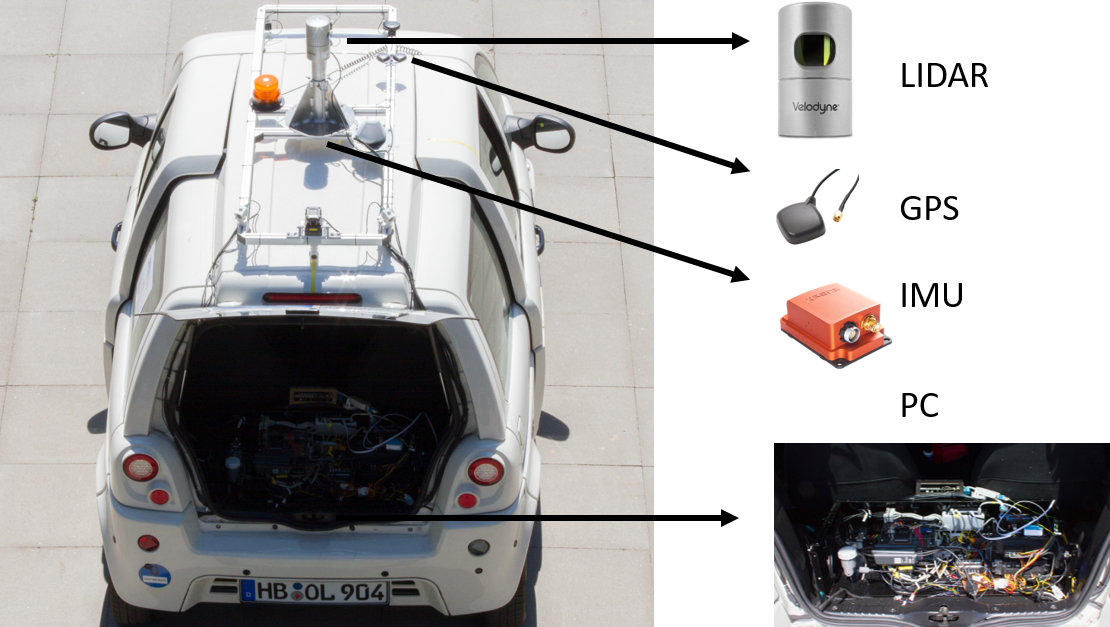
\includegraphics[scale=0.6]{mia2}
    \caption{Sensor setup configuration on MIAcar}
    \label{fig:setup}
\end{figure}


\newpage
Alternatively, we also tested these algorithms with another dataset which is called KITTI (Karlsruhe Institute of Technology and Toyota Technological Institute). This data set is promoted as a benchmark to validate any localization algorithms \cite{kitti}.
\par To continue, we organized this chapter as follows: In Section \textbf{\ref{sec:Exp}}, we explained the experimnetal setups and show the preliminary works. We then presented the results  of MIA and KITTI in Section \textbf{\ref{sec:MIA-set}} and \textbf{\ref{sec:KITTI-set}}, respectively.

\section{Experimental Procedure}\label{sec:Exp}
To cover different aspects of real-world conditions, experiments should be designed in a wide spectrum. Therefore, we conducted several experiments in different environments and different weather conditions as much as possible. However, we must do some preparations which are always need to be considered in order to conduct a proper experiment. For this reason, we described the required works in the following section. 

\subsection{Preliminary Work}
\subsection*{Sensor Positioning} 
The first task was to determine the position of sensors w.r.t center of the vehicle, in particular, LIDAR and IMU. Since the main localization algorithm that used in this thesis affiliates with LIDAR and IMU, thereby the position of these sensors had a big impact on results. Thus, the preliminary works on these sensors setup highly important in order to have concrete results from localization algorithms and having an accurate 3D map.
\subsection*{Map Construction}\label{mapping}
Once the positions of sensors were determined and set them up correctly, the second work was to build a map of the environment where the experiment would be carried out. For this purpose, the car was first driven in a test area to collect the related sensory data e.g. point clouds for creating a three-dimensional map as shown in figure \ref{fig:rh_3d}.
\par To create 3D map, we used NDT algorithm in the same manner as mentioned in \cite{ndt_map}. The working principle of NDT is almost the same as the localization algorithm, except it saves every scan match in space instead. Of note, this method is very time intensive for building map even though it provides a relatively accurate map. Nevertheless, the created map was used for the course of this thesis.

\begin{figure}[t!]
\subfloat[3D Map of Robert-Hooke-Straße in Bremen \label{fig:rh_3d}] {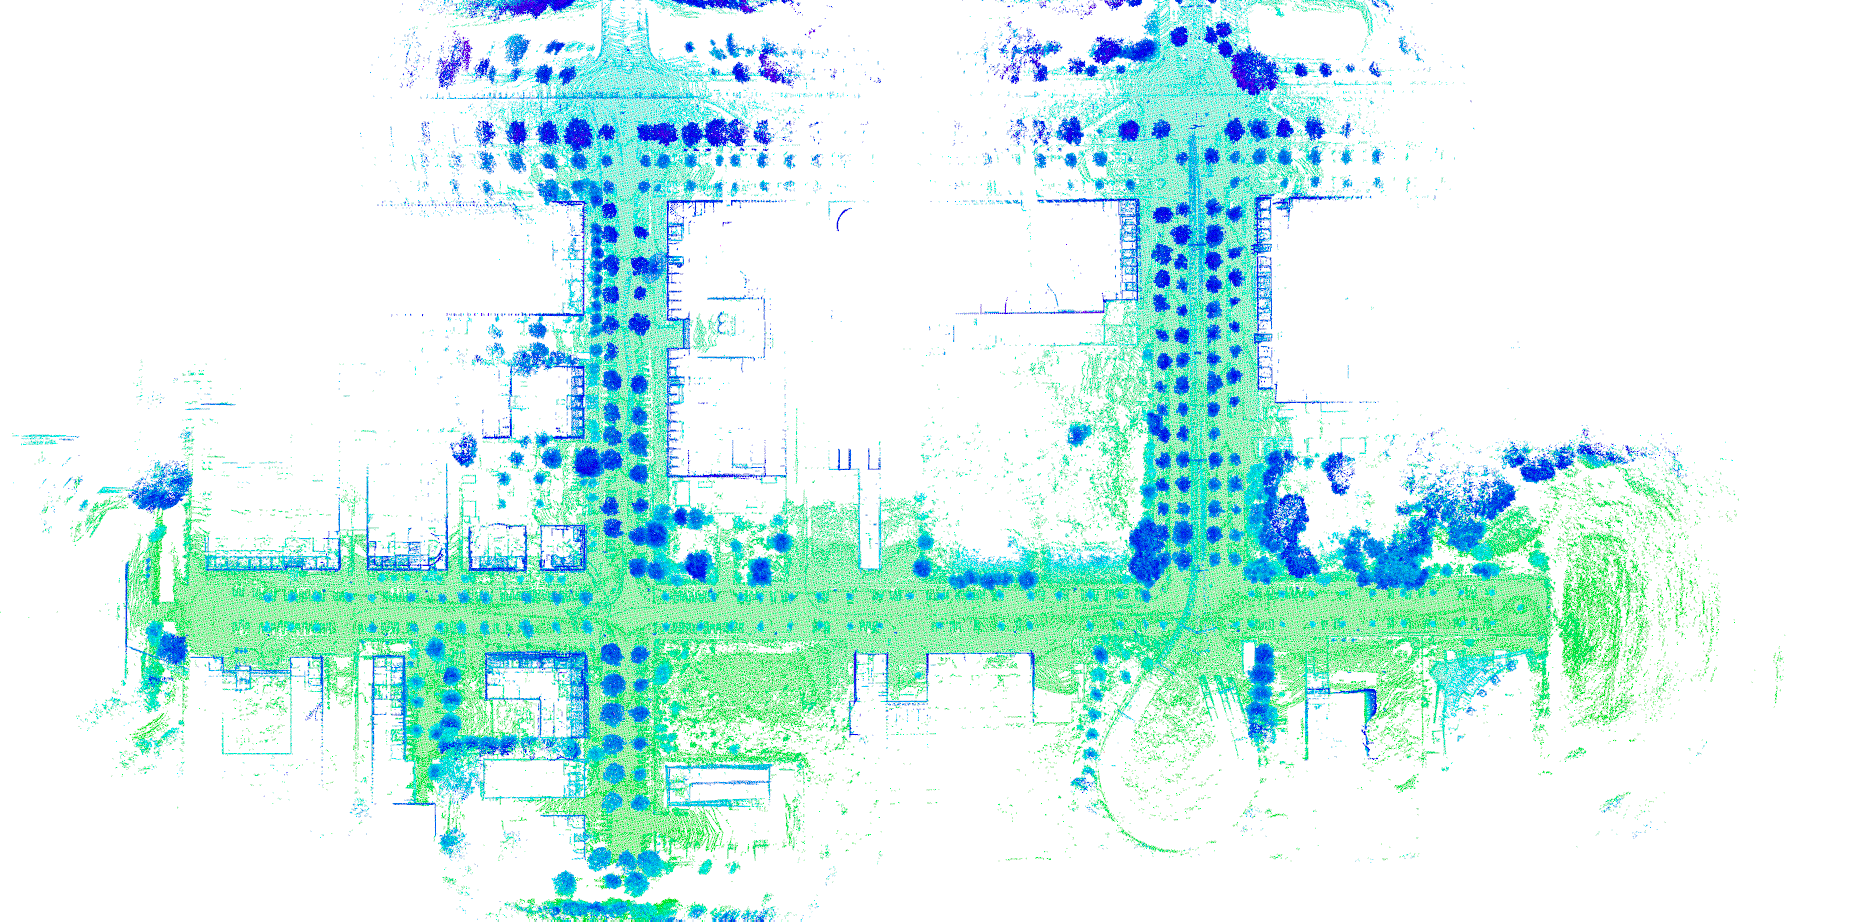
\includegraphics[width=\textwidth]{rh_3d}}\\
\subfloat[The bird view of Robert-Hooke-Straße in Bremen \label{fig:rh_google}]{\includegraphics[width=\textwidth]{rh5_google}}
\label{fig:comparison}
\caption{Comparing the created 3D map (a) and real map (b)}
\end{figure}

\newpage
\subsection*{Down Sampling}
The final task was concerning to decrease the computational time of the map-based localization algorithm. As it was previously discussed, the most preferable way to keep the execution time in optimum level is to down-sample both data that obtained from map and LIDAR. By this way, we also decreases the complexity of the map and distribute LIDAR points evenly (see figure \ref{fig:vox_size}) \cite{ndt_map}. In figure \ref{fig:no_filter}, the map contains a large amount of redundant information i.e. the surface of objects in the map are represented by a set of points that are more than needed to depict the surface of the object. Therefore, the original map was needed to be down-sampled as shown in figure \ref{fig:filter_rh}.

\begin{center}
\begin{figure}
\subfloat[\textbf{Original Map:} 3D map of the area was generated (offline) from recorded LIDAR sensor data. It contains 71,120,230 points of 1GB size.
\label{fig:no_filter}] {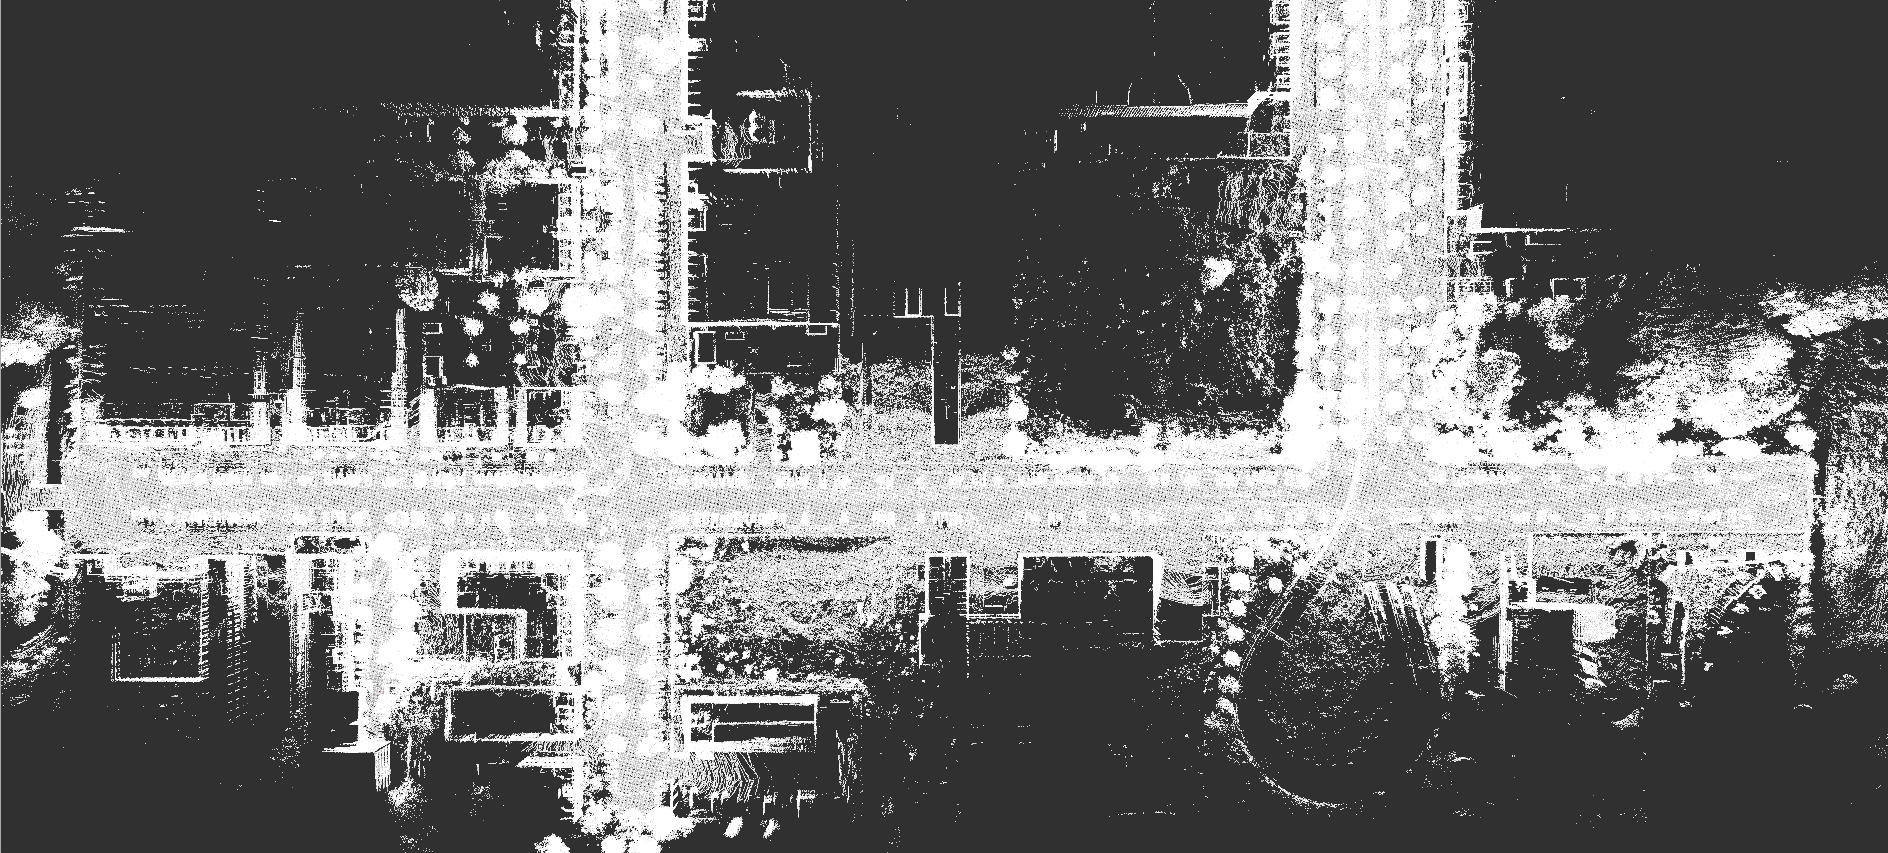
\includegraphics[scale=0.3]{no_filter}}\\
\subfloat[\textbf{Down-sampled Map:} After down-sampled process (filter size 0,5m), map contains 1,110,350 points of 17,8MB size \label{fig:filter_rh}]{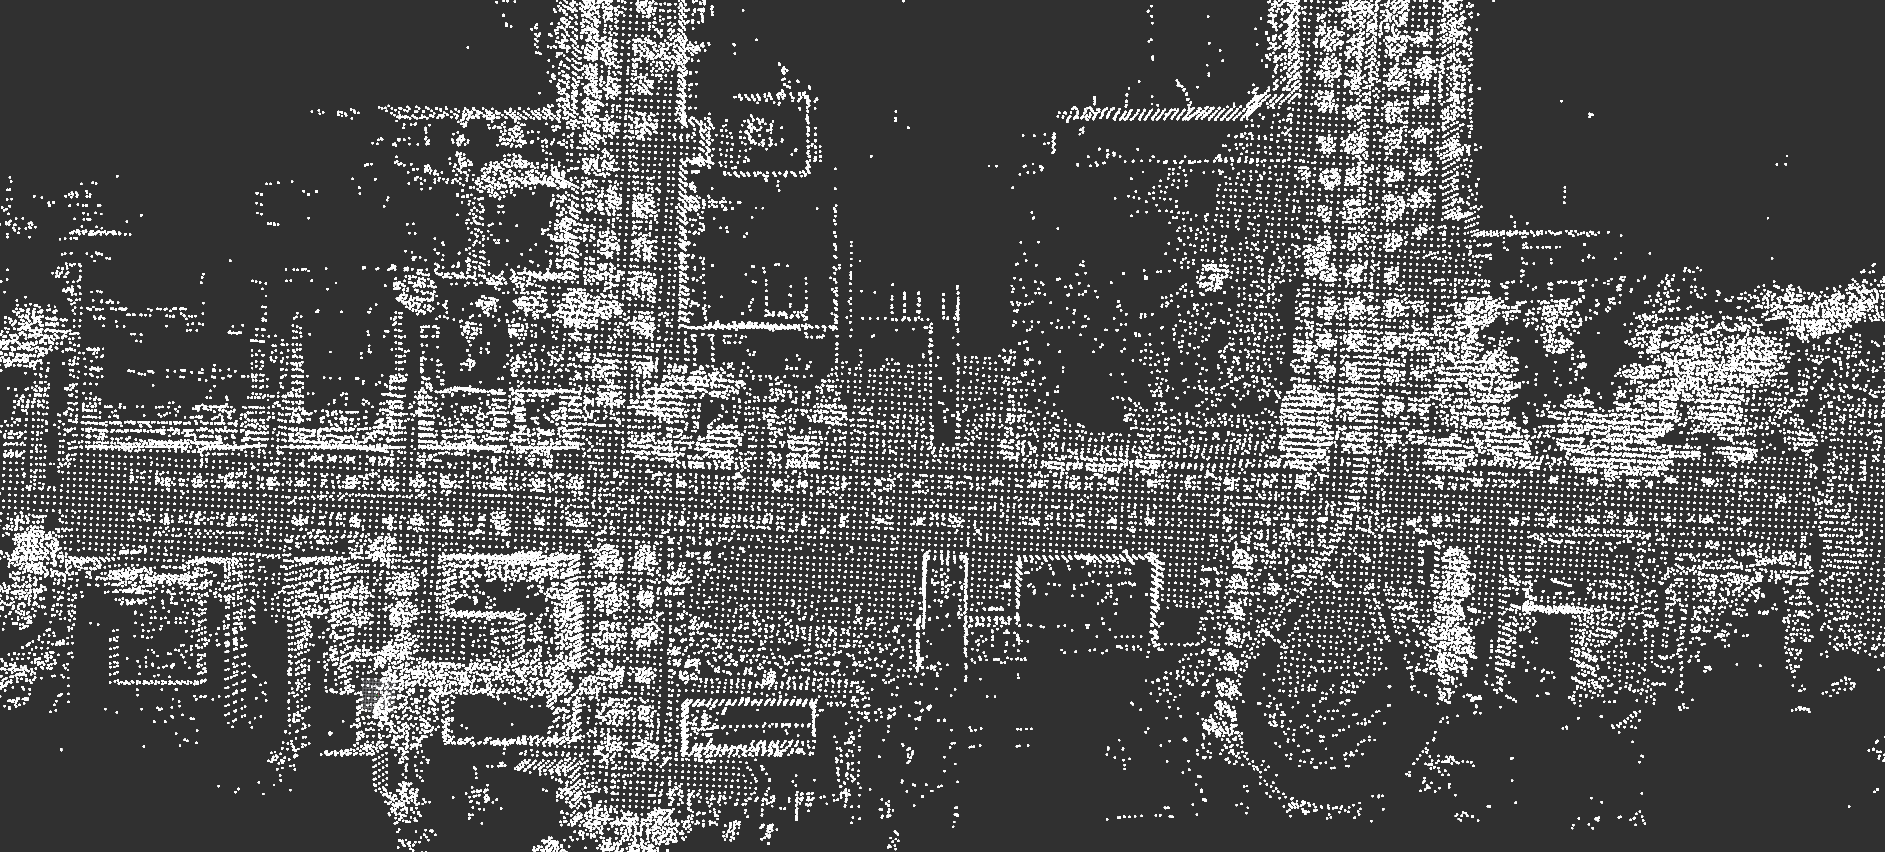
\includegraphics[scale=0.3]{filtered_rh}}
\label{fig:filter}
\caption{Illustration of orginal map (a) and down-sampled map (b) }
\end{figure}
\end{center}

\begin{figure}[t]
\subfloat[Voxel size = 0 m]{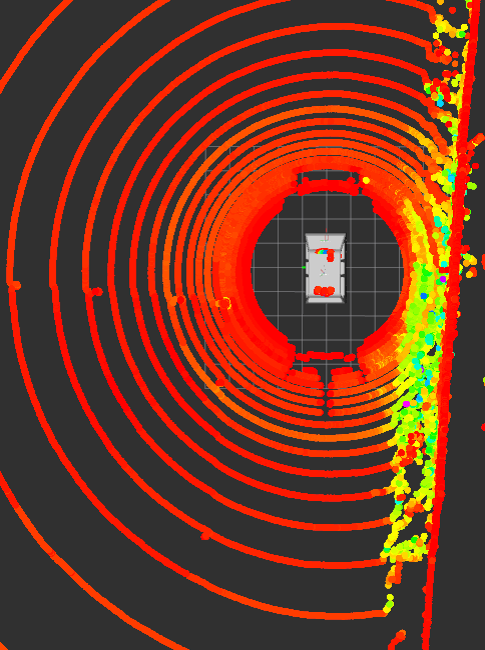
\includegraphics[scale=0.5]{0}}\hfill
\subfloat[Voxel size = 1 m]{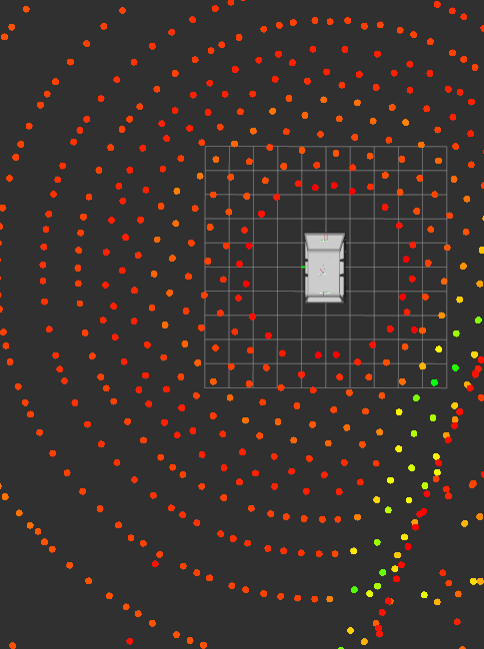
\includegraphics[scale=0.5]{1}}\hfill
\subfloat[Voxel size = 2 m]{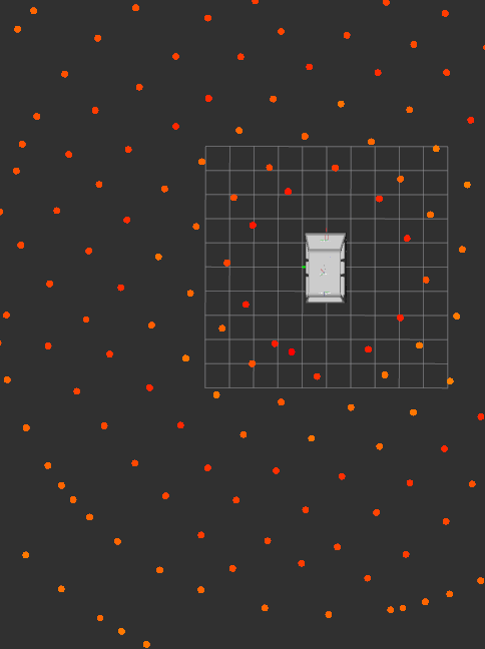
\includegraphics[scale=0.5]{2}}\\
\subfloat[Voxel size = 3 m]{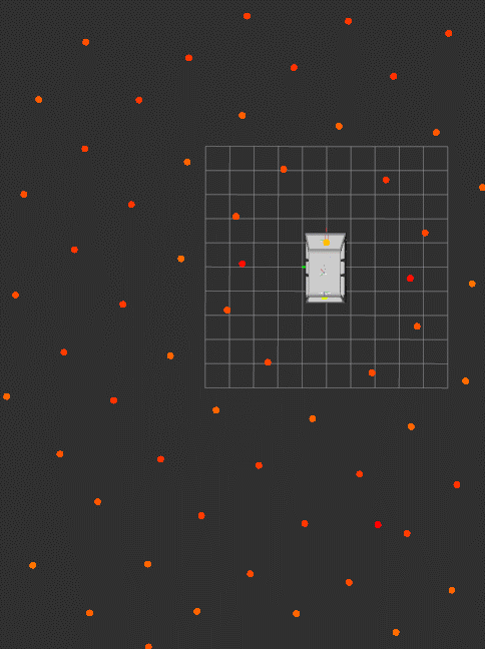
\includegraphics[scale=0.5]{3}}\hfill
\subfloat[Voxel size = 4 m]{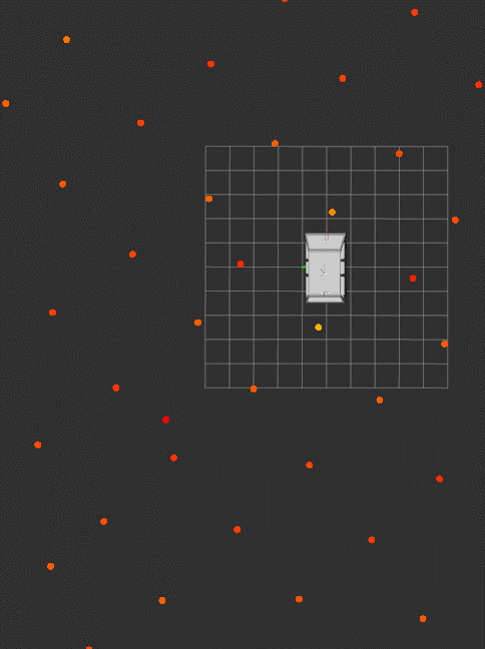
\includegraphics[scale=0.5]{4}}\hfill
\subfloat[Voxel size = 5 m]{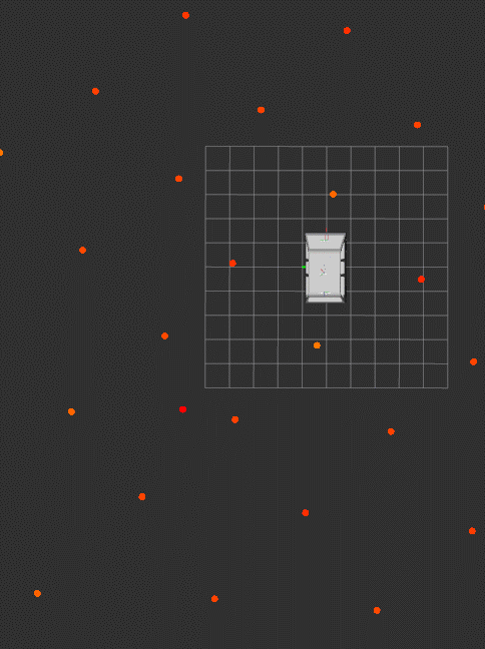
\includegraphics[scale=0.5]{5}}\hfill
\caption{Distribution of laser points over the different size of voxel}
\label{fig:vox_size}
\end{figure}
\vspace{-1cm}
\par To down-sample, we used an algorithm that was provided by \acrfull{ros} is Voxel-filter\footnote{\url{http://wiki.ros.org/pcl_ros}}%comment:The VoxelGrid class creates a 3D voxel grid (think about a voxel grid as a set of tiny 3D boxes in space) over the input point cloud data. Then, in each voxel (i.e., 3D box), all the points present will be approximated (i.e., downsampled) with their centroid. This approach is a bit slower than approximating them with the center of the voxel, but it represents the underlying surface more accurately.
. The concept of this filter is to find the centroid of points $(C_{x}, C_{y})$ within voxel cell as described in the following equations:\\
\begin{equation}
C_{x} =\dfrac{1}{6A}\sum_{i=0}^{n-1}(x_{i}+x_{i+1})(x_{i}y_{i+1}-x_{i+1}y_{i})
\end{equation}
\begin{equation}
C_{y} =\dfrac{1}{6A}\sum_{i=0}^{n-1}(y_{i}+y_{i+1})(x_{i}y_{i+1}-x_{i+1}y_{i})
\end{equation}\\
and where A is the polygon's signed area as described by \cite{centroid},
\begin{equation}
A =\dfrac{1}{2}\sum_{i=0}^{n-1}(x_{i}y_{i+1}-x_{i+1}y_{i})
\end{equation}

\section{MIA Dataset}\label{sec:MIA-set}
MIA dataset was  created by driving the car around Robert-Hooke-Straße, Jeddeloh driver training area and Bassum go-kart track. Dataset consist of LIDAR, IMU, wheel rotation, RGB image and radar information.
\subsection{Robert-Hooke-Straße Test} The first test was carried out in a place where the road condition was asphalt and the weather was sunny. The vehicle was driven around in this place approximately \textbf{2167} meter (m) (see figure \ref{fig:rh_gps}) and the result of algorithms was evaluated by collected raw data.
\\
\begin{figure}[ht]
    \centering
    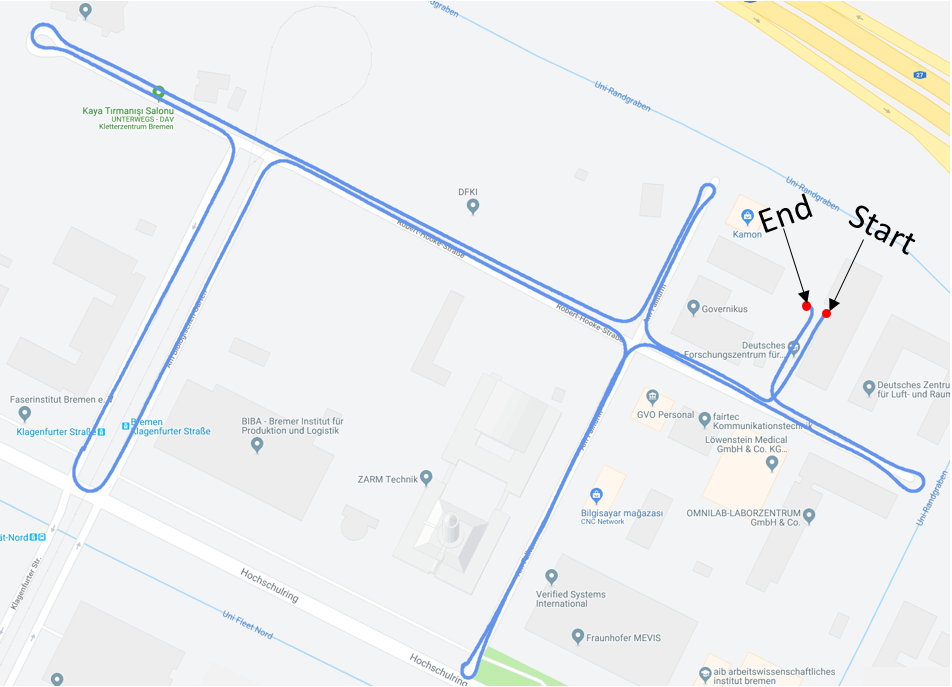
\includegraphics[scale=0.50]{rh_gps}
    \caption{The bird view of the first test area. The vehicle was driven manually for data acquisition on the blue line which indicates the GPS trace}
    \label{fig:rh_gps}
\end{figure}

\noindent \textbf{Assessment of the Idea:} All the obtained result including translations and rotations errors were evaluated by comparing them with ground truth which was obtained via NDT algorithm under the following conditions:
\begin{itemize}
    \item Map resolution 0.2 m,
    \item Source resolution 1 m.
\end{itemize}

As seen on the plots below, pure wheel odometry (a) and improved odometry (b) described in \ref{sec:wheel_odometry} were compared with the ground truth. It is quite clear that using heading velocity from IMU sensor enhances the quality of the wheel odometry about \textbf{30} \%. Nevertheless, error of wheel odometry was more larger than  upper limit for autonomous driving. On the graph \ref{fig:odom_compare_all}, we presented overall comparison between odometry and the ground truth.
\begin{figure}[H]
\centering
\subfloat[\small Performance of pure wheel odometry against ground truth in 3D showed as translation and rotation errors]{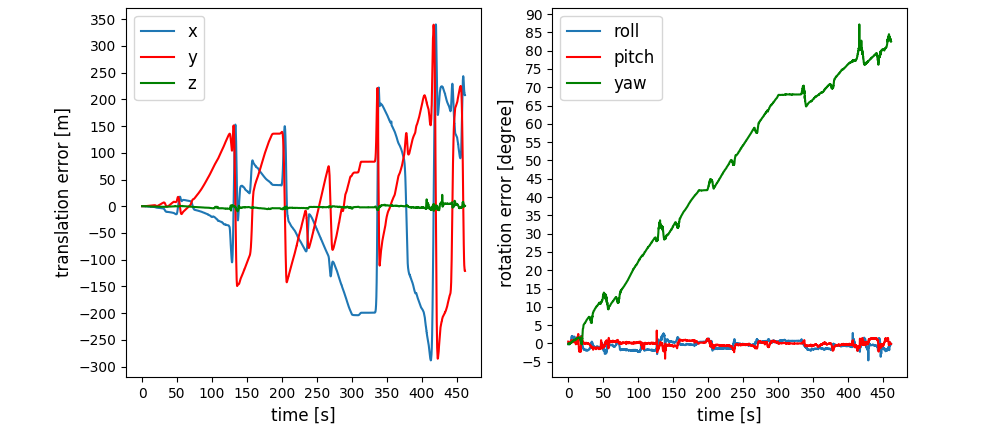
\includegraphics[height=5cm,width=\textwidth]{odom_error}}\\
\subfloat[\small Performance of wheel odometry with IMU against ground truth in 3D showed as translation and rotation errors]{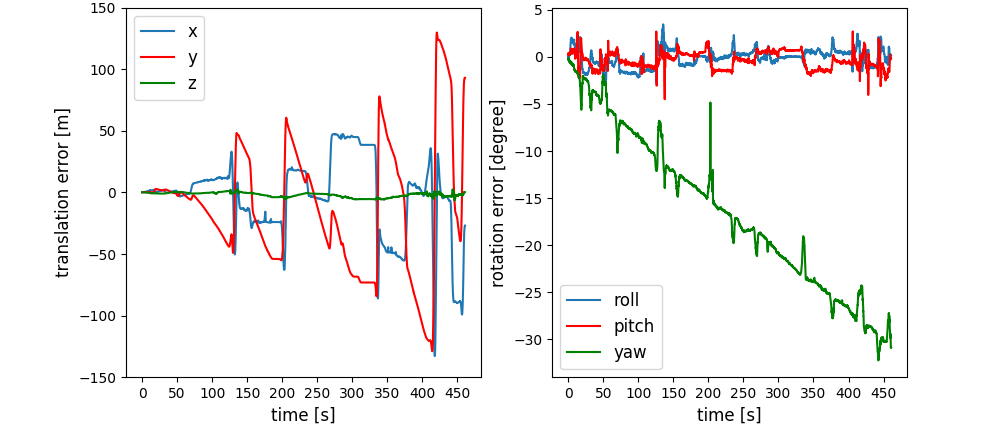
\includegraphics[height=5cm,width=\textwidth]{odom_imu_error}}
\label{fig:wheel_compare}
\end{figure}
\vspace{-0.5cm}
\begin{figure}[H]
    \centering
    \subfloat[\small {Overall comparison between ground truth (blue), steering-wheel-based wheel  odometry(red) and IMU-based wheel odometry (green)}]{\label{fig:odom_compare_all}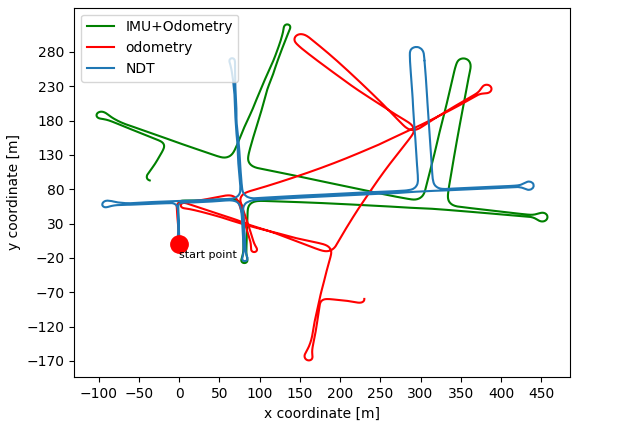
\includegraphics[scale=0.4]{ndt_imu_odom_compare.png}}
    \caption{Comparison between odometry and ground truth}
    \label{fig:my_label}
\end{figure}

\par Next task was improving wheel odometry by fusing IMU and GPS data. For this purpose, the performance of EKF was tested by integrating linear and heading velocity ($V_x, V_y, \dot{\theta}$), x-y positions, angular velocities ($\dot {roll}, \dot {pitch}, \dot {yaw}$) and acceleration ($\ddot X, \ddot Y, \ddot Z$) from wheel odometry, GPS and IMU, respectively. 
\begin{figure}[H]
    \centering
    \subfloat[General view of comparison between EKF (red) and ground truth (blue)]{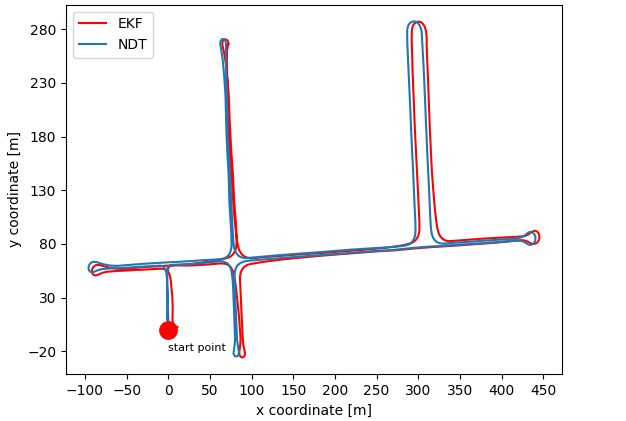
\includegraphics[scale=0.4]{ekf_vs_ndt}\label{fig:ekf_vs_ndt}}
\end{figure}
\vspace{-0.5cm}
\begin{figure}[H]
    \centering
    \subfloat[\small{Performance comparison between EKF together with GPS, IMU, Odometry and ground truth in 3D showed as translation and rotation errors }]{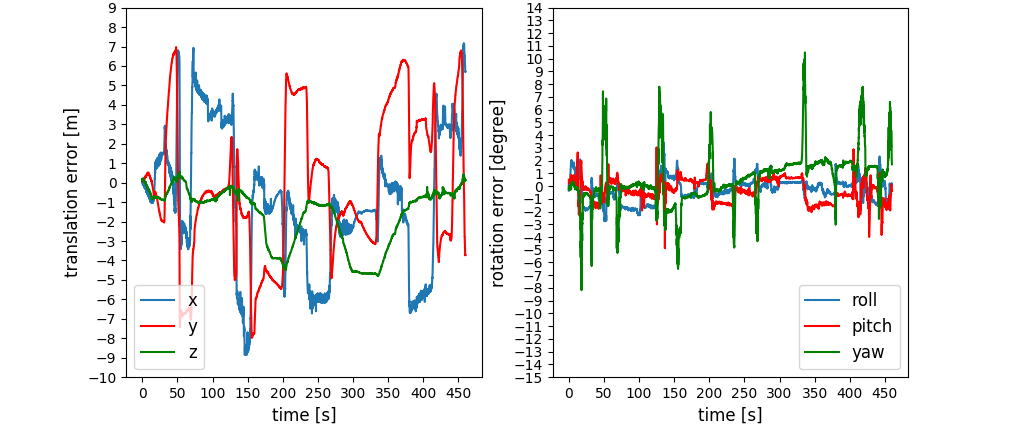
\includegraphics[height=5cm,width=\textwidth]{ekf_error}\label{fig:ekf_error}}
    \caption{Comparison between EKF and ground truth}
    \label{fig:ekf_graph}
\end{figure}
\noindent Despite good performance (see figure \ref{fig:ekf_graph}) of EKF compared with previous example, the overall performance of EKF was not as precise as the ground truth as shown figure \ref{fig:ekf_vs_ndt}.

\par Before proceeding the final test, we had to make a decision between two scan registration methods to have more efficient and robust localization. Therefore, we conducted another test to evaluate their performance against each other in terms of execution time, translation, and rotation differences.\\ 
\par Of note, to make a fair test, we should use the same map whose voxel size 2 m. However, we found out that NDT algorithm cannot handle sparse map, while ICP worked much more successfully. In contrast, ICP could not make any progress on a relatively intensive map, while NDT worked seamlessly. Thus, we had to use two different maps but we set the common parameters of two methods exactly the same to keep the test as fair as possible.
\begin{itemize}
\item Common parameters
\begin{itemize}
    \item down-sampled source scan (LIDAR) by 2m voxel size,
    \item same initial translation and rotation error (both initialized by GPS),
    \item same number of iterations 50.
\end{itemize}
\end{itemize}

\begin{figure}[H]
\centering
\subfloat[General view of comparison between ICP (red) and NDT (blue), in side of the boxes the overlap showed at higher magnification]{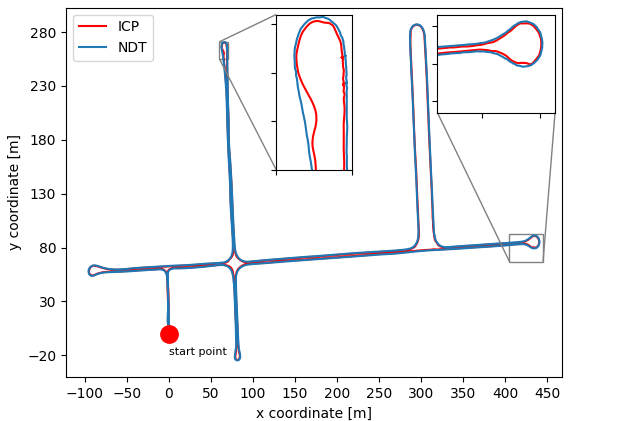
\includegraphics[scale=0.4]{icp_vs_ndt}\label{icp_mag}}
\end{figure}
\vspace{-0.5cm}
\begin{figure}[H]
\centering
\subfloat[Performance comparison between NDT and ICP in 3D showed as translation and rotation error ]{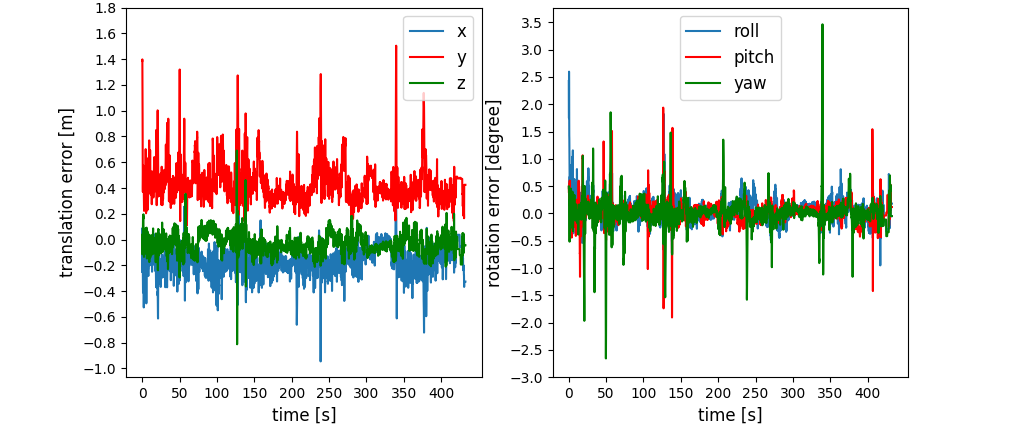
\includegraphics[height=5cm,width=\textwidth]{error_icp}}
\caption{Comparison between two scan registration algorithm NDT and ICP}
\label{fig:icp_vs_ndt}
\end{figure}
\begin{table}[H]
    \centering
    \small
    \begin{tabular}{|c|c|c|c|}
    \hline
         methods &resolution of map [m]&filter size of source [m]&exec. time [s]\\ 
         \hline
         ICP& 2& 2 & 89.80\\
         \hline
         NDT& 0.2 & 2 & 31.63\\
         \hline
    \end{tabular}
    \caption{Execution time of methods under the certain condition}
    \label{tab:compare_ekf_ndt}
\end{table}

It is fairly clear that ICP has a tendency to go inside to keep the overlap area as much as it can ( seen figure \ref{icp_mag}). It also can be clearly seen that ICP could not find the proper transformation as good as NDT between target and source scan when the vehicle made u-turn. Another aspect of this comparison is observing the execution time of both methods which was stated in table \ref{tab:compare_ekf_ndt} under the certain conditions such as map resolution and filter size. The execution time is playing a distinct role in deciding to which method used primarily for supplying proper localization less 100 ms since it is the sampling time of the LIDAR sensor.

\newpage
\par Finally, we tested the method as shown in figure \ref{fig:ndt_son}, which combines the EKF with NDT, under the following condition:
\begin{itemize}
    \item Map resolution 0.75 m,
    \item Source resolution 3 m,
    \item initial state of EKF 0.5 m $x$, 0.05 m $y$ and -0.03 rad $\theta$
\end{itemize}
By doing this, we aimed to make NDT methods less sensitive about the density of map and to eliminate any possible fluctuation on localization (see figure \ref{fig:ekf_ndt_vs_ndt}).

\begin{figure}[H]
\centering
\subfloat[General view of comparison between combination of EKF with NDT (red) and NDT (blue), in side of the boxes  the elimination of vibration showed at higher magnification]{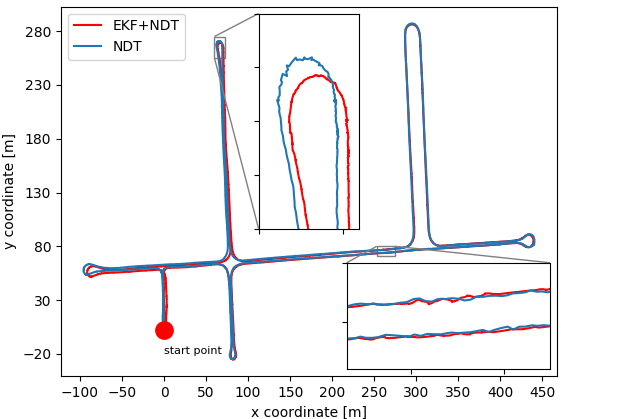
\includegraphics[scale=0.4]{ekf_ndt_vs_ndt}}
\end{figure}
\vspace{-0.5cm}
\begin{figure}[H]
\subfloat[Performance comparison between combination of EKF with NDT and NDT in 3D showed as translation and rotation errors]{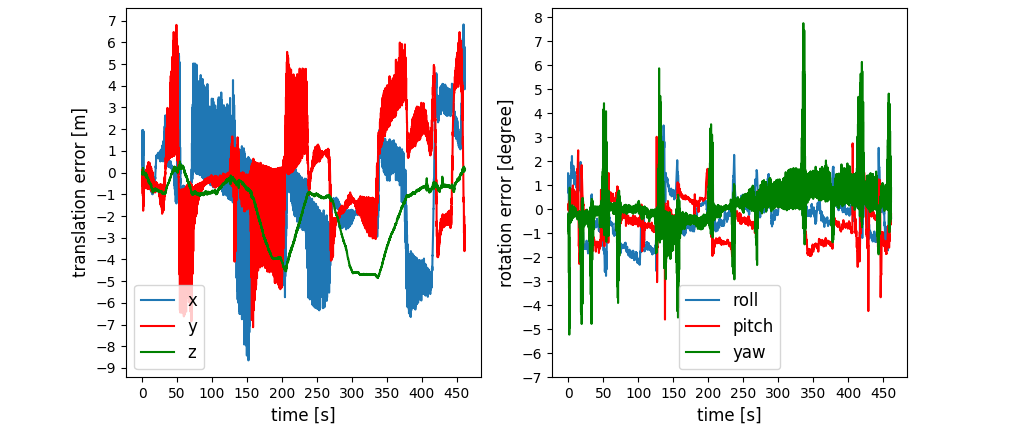
\includegraphics[height=5cm,width=\textwidth]{error_ekf_ndt_vs_ndt}\label{error_ekf_ndt}}
\caption{Comparison between combination of EKF with NDT and NDT}
\label{fig:ekf_ndt_vs_ndt}
\end{figure}

\begin{table}[H]
    \centering
    \small
    \begin{tabular}{|c|c|c|c|c|c|}
    \hline
         translation &max e.[m]&RMSE[m]&rotation&max e. [deg]&RMSE[deg]\\ 
         \hline
         x &8.65114&2.44113& roll  &3.48991&0.94101\\
         \hline
         y &7.12333&2.26043& pitch &4.59713&0.93819\\
         \hline
         z &4.85689&2.27955& yaw   &7.74988&0.99059\\
         \hline
    \end{tabular}
    \caption{Error calculation data which was subtracted from figure \ref{error_ekf_ndt}}
    \label{tab:compare_ekf_icp}
\end{table}
Additionally, we tested the combination of EKF with ICP as shown in the plots below.
\begin{figure}[H]
\centering
\subfloat[General view of comparison between combination of EKF with ICP (red) and ICP (blue), in side of the boxes  the elimination of vibration showed at higher magnification]{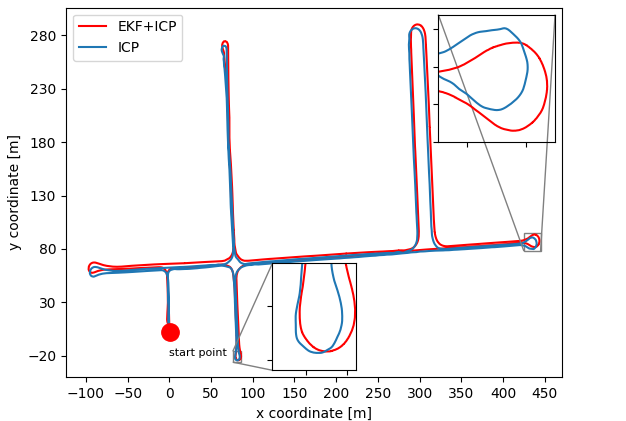
\includegraphics[scale=0.4]{ekf_icp_vs_icp}}
\end{figure}
\vspace{-0,5cm}
\begin{figure}[H]
\subfloat[Performance comparison between combination of EKF with ICP and NDT in 3D showed as translation and rotation error]{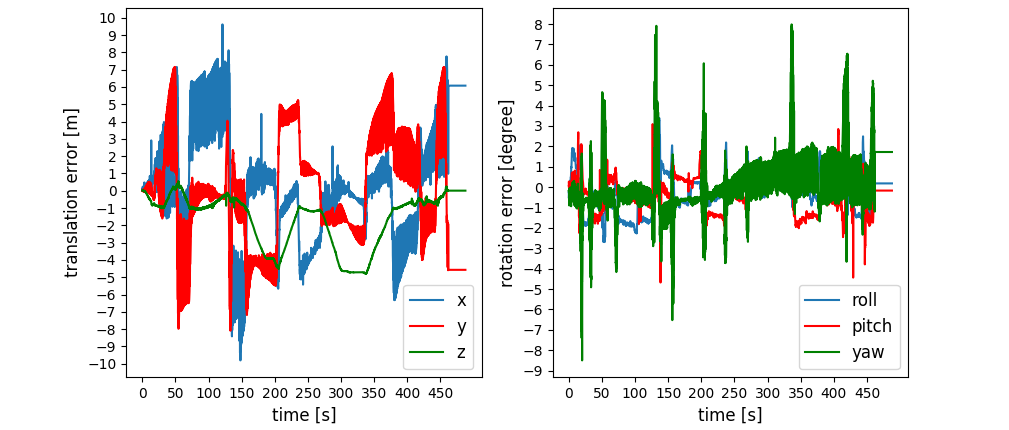
\includegraphics[height=5cm,width=\textwidth]{error_ekf_icp_vs_ndt}\label{error_ekf_icp}}
\caption{Comparison between combination of EKF with ICP and ICP}
\label{fig:ekf_icp_vs_icp}
\end{figure}

\begin{table}[H]
    \centering
    \small
    \begin{tabular}{|c|c|c|c|c|c|}
        \hline
         translation &max e.[m]&RMSE[m]&rotation&max e. [deg]&RMSE[deg]\\          \hline
         x &9.80437&3.60233& roll  &3.39731&0.92542\\
         \hline
         y &8.08773&3.42366& pitch &4.68054&0.91935\\
         \hline
         z &4.79653&2.21747& yaw   &8.50213&1.68752\\
         \hline
    \end{tabular}
    \caption{Error calculation data which was subtracted from figure \ref{error_ekf_icp}}
    \label{tab:exec_time}
\end{table}
\noindent EKF has done its task to eliminate all possible fluctuations on localization data. However, as it seen in figure \ref{fig:ekf_ndt_vs_ndt} and \ref{fig:ekf_icp_vs_icp}, there is a difference between EKF result and ground truth due to improper use of Kalman parameters. Table \ref{tab:compare_ekf_icp} and \ref{tab:exec_time} show the error calculation in term s of absolute maximum and mean translation and rotation error.
\subsection{Jeddeloh driver training area Test} The second test was carried out in a place where the road condition was gravel and weather was drizzle. The vehicle was driven in this place approximately 796 m (see figure \ref{fig:jeddeloh_gps}) and the obtained results of the algorithms was evaluated in the same manner as the previous example.
\\
\begin{figure}[H]
    \centering
    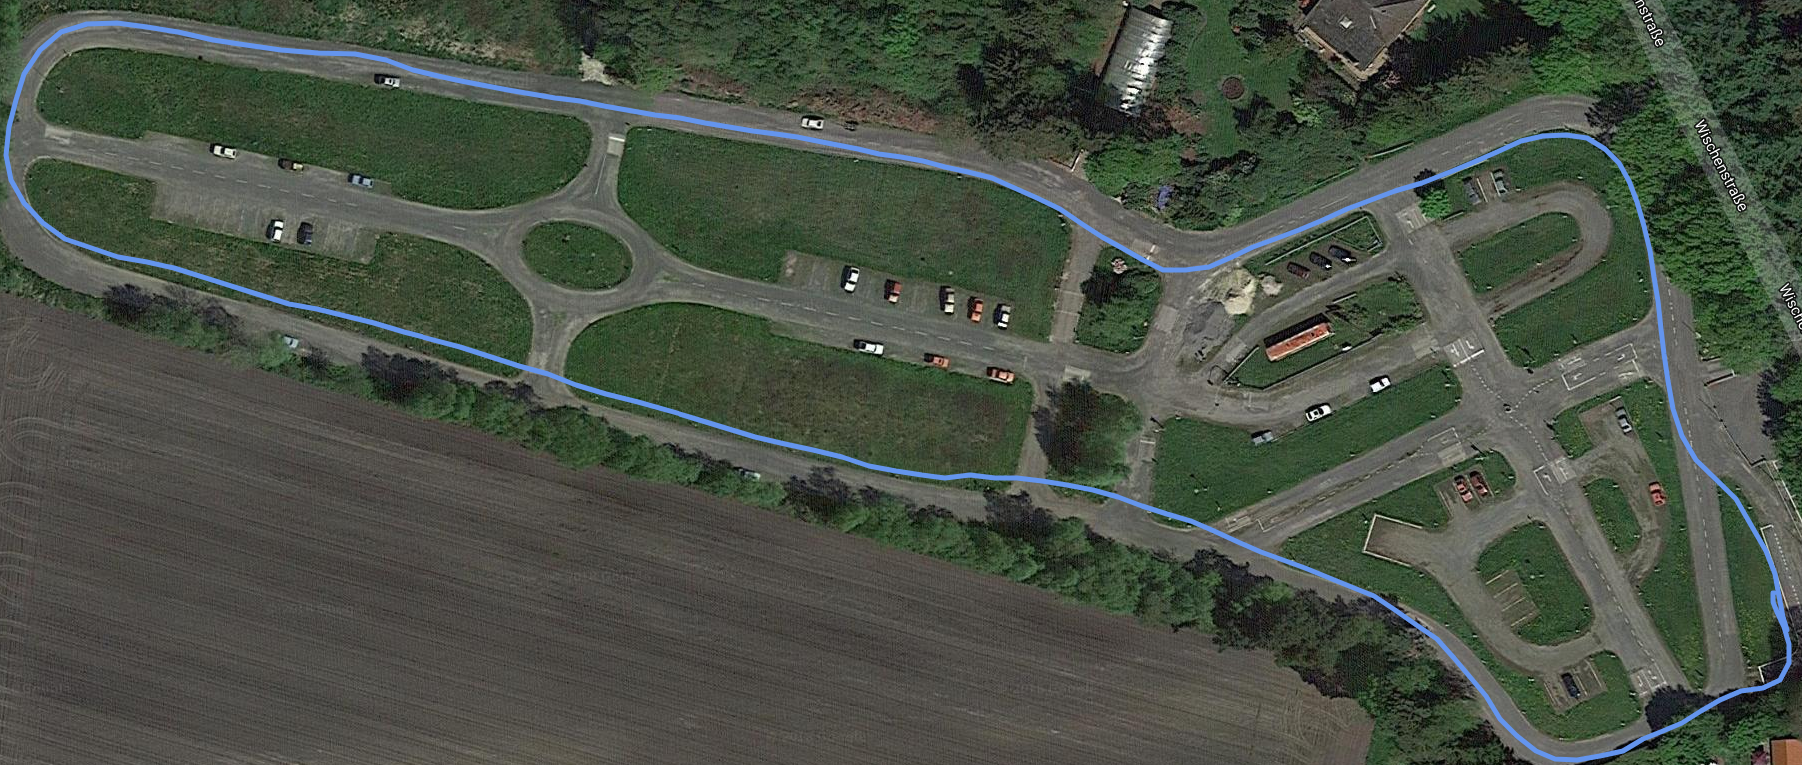
\includegraphics[scale=0.23]{jeddloc_gps}
    \caption{The bird view of the second test area. The vehicle was driven manually for data acquisition on the blue line which indicates the GPS trace}
    \label{fig:jeddeloh_gps}
\end{figure}
\noindent\textbf{Assessment of the Idea:} In this part, we only presented the final result which was provided by the combination EKF with NDT  as shown in figure \ref{fig:jeddeloh_error}. 
In this experiment, we realized that the process and measurement noise co-variance matrices of EKF was needed to be reconfigured due to the different road condition that was chosen for this experiment. Since the vehicle was driven on uneven terrain, in our case the it was gravel, it has a great impact on the measurement of the wheel odometry and IMU. In this sense, we chose Q smaller than the previous example in order to mitigate this effect. As a result of this, the combination of EKF with NDT algorithm delivered a relatively good result as stated in table \ref{tab:jeddeloh}. 
\\
\begin{figure}[H]
    \centering
    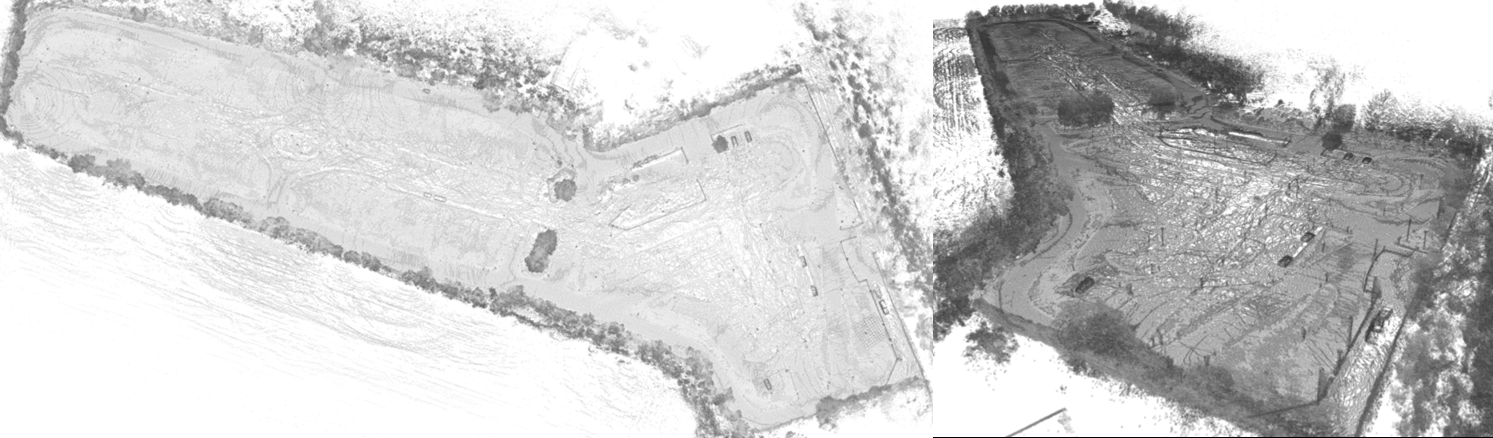
\includegraphics[width=\textwidth]{gray_jeddeloh.png}
    \caption{3D map of Jeddeloh Test area which was constructed by NDT-algorithm}
    \label{fig:3D_jeddeloh}
\end{figure}

\begin{center}
\begin{figure}
\centering
\captionsetup[subfigure]{justification=centering}
\subfloat[General view of comparison between combination of EKF with NDT (red) and NDT (blue)]{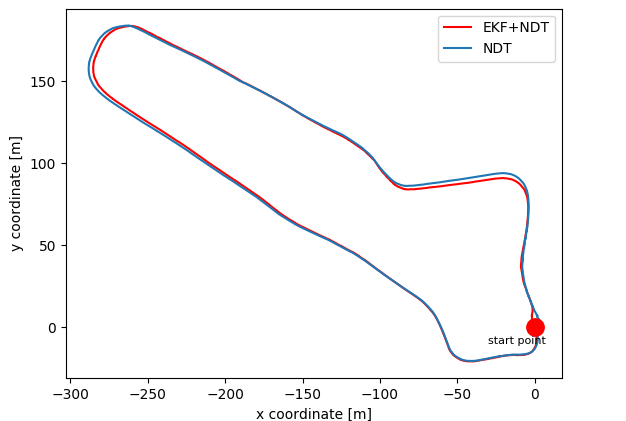
\includegraphics[scale=0.4]{jeddeloh_ekf_ndt}\label{fig:jeddeloh_ekf}}\\
\subfloat[Performance comparison between combination of EKF with NDT and NDT in 3D showed as translation and rotation error]{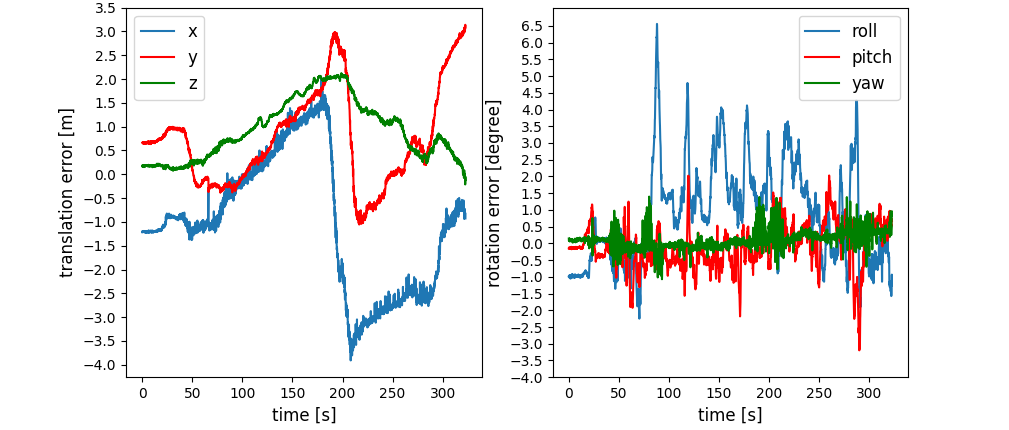
\includegraphics[height=5cm,width=\textwidth]{jeddeloh_error.png}\label{fig:jeddeloh_errorb}}
\caption{Comparison between combination of EKF with NDT and ground truth}
\label{fig:jeddeloh_error}
\end{figure}

\begin{table}
    \centering
    \small
    \begin{tabular}{|c|c|c|c|c|c|}
        \hline
         translation &max e.[m]&RMSE[m]&rotation&max e. [deg]&RMSE[deg]\\          
         \hline
         x &3.90913&1.74429& roll &6.55794&1.72251\\
         \hline
         y &3.13895&1.25324& pitch &3.19698&0.68359\\
         \hline
         z &2.19162&1.12061& yaw &1.39722& 0.30418\\
         \hline
    \end{tabular}
    \caption{Error calculation data which was subtracted from figure \ref{fig:jeddeloh_errorb}}
    \label{tab:jeddeloh}
\end{table} 
\end{center}

\newpage
\subsection{Bassum Go-kart race track Test} \label{sub:Bassum} The final test was conducted in the Bassum go-kart place and the localization algorithm was tested while the vehicle was autonomously driven.

\begin{figure}[H]
    \centering
    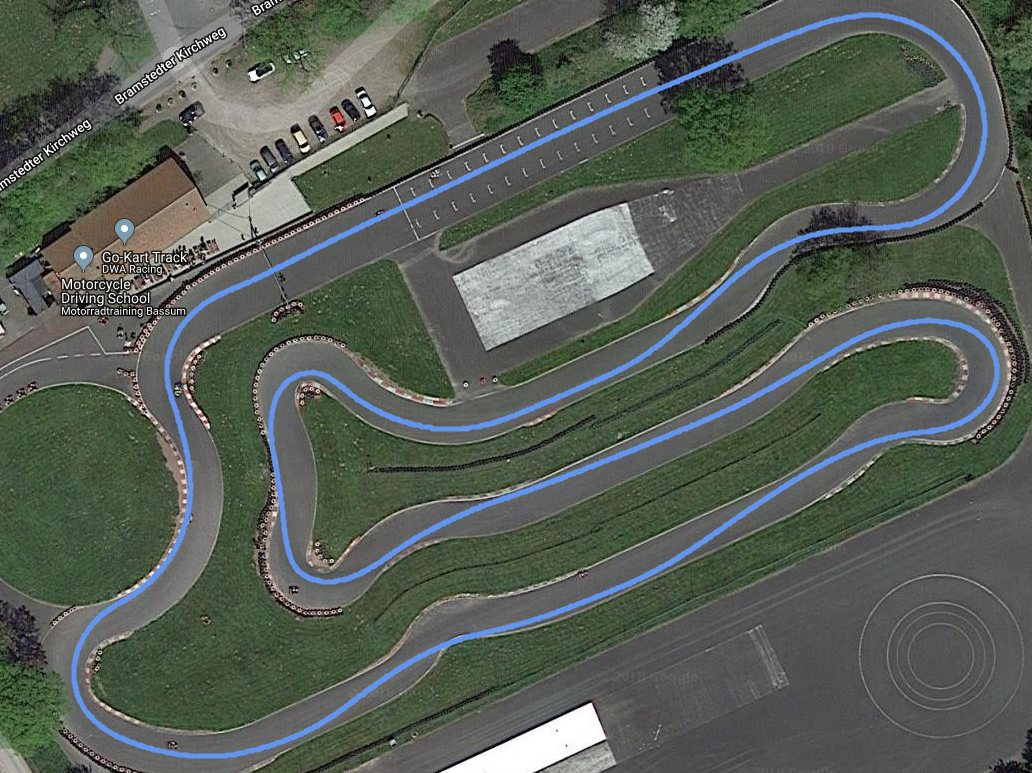
\includegraphics[scale=0.32]{bassum_gps}
    \caption{The bird view of the third test area. The vehicle was driven autonomously on the blue line which indicates the trajectory}
    \label{fig:bassum_gps}
\end{figure}
\noindent\textbf{Assessment of the Idea:} Since the real trajectory has no information about height, roll, and pitch, the evaluation was done by comparing only translation error in 2D x,y and rotation error w.r.t z-axis between NDT and the real trajectory. On the graphs above show the result of the NDT localization algorithm under the optimal circumstance, using a map and source whose resolution 0.2m and 3m, respectively. Therefore, the maximum translation/rotational error of the algorithm smaller than 0.4 m/deg, as stated in the table \ref{tab:bassum}.
\begin{figure}[H]
    \centering
    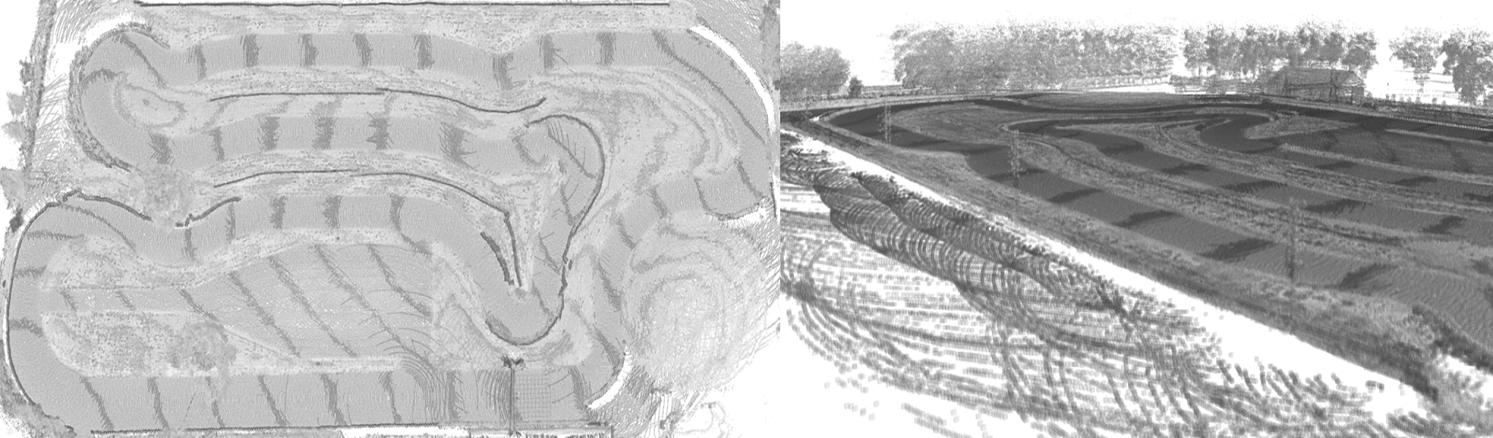
\includegraphics[width=\textwidth]{gray_bassum.png}
    \caption{3D map of Bassum Test area which was constructed by NDT-algorithm}
    \label{fig:3D_bassum}
\end{figure}

\begin{figure}[H]
    \centering
    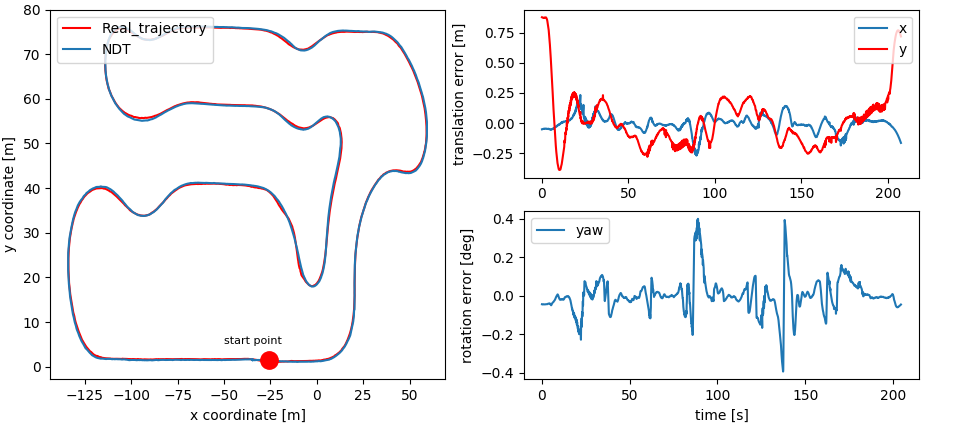
\includegraphics[height=5cm,width=\textwidth]{bassum_overall}
    \caption{NDT localization performance was shown against reference(real) trajectory comparing with translation and rotation error }
    \label{fig:bassum_overall}
\end{figure}
\vspace{-10pt}
\begin{table}[H]
    \centering
    \small
    \begin{tabular}{|c|c|c|c|c|c|}
        \hline
         translation &max e.[m]&RMSE[m]&rotation&max e. [deg]&RMSE[deg]\\  
         \hline
         x &0.21895&0.00184 & roll &-& -\\
         \hline
         y &0.37582&0.01251 & pitch & -& -\\
         \hline
         z &-&- &yaw &0.35267& 0.00118\\
         \hline
    \end{tabular}
    \caption{Error calculation data which was subtracted from figure \ref{fig:bassum_overall}}
    \label{tab:bassum}
\end{table}

\newpage
\section{KITTI Dataset}\label{sec:KITTI-set}
This section was conducted by \acrfull{kitti} data set, which is provided by KITTI. It was used to verify the results of our localization algorithms. Even though the KITTI data of interest is visual odometry, optical flow and etc., provided data set is showing similarity with our data set in terms of used sensors such as IMU, GPS, LIDAR, RGB and gray cameras except only for wheel odometry. Therefore, the KITTI dataset was utilized to compare the outputs of the localization methods with KITTI ground truth that is provided by D-GPS. In following, we presented the result of the combination of EKF with NDT by using sequence number 10 KITTI data which is shown in figure \ref{fig:kitti_gps}.

\begin{figure}[H]
    \centering
    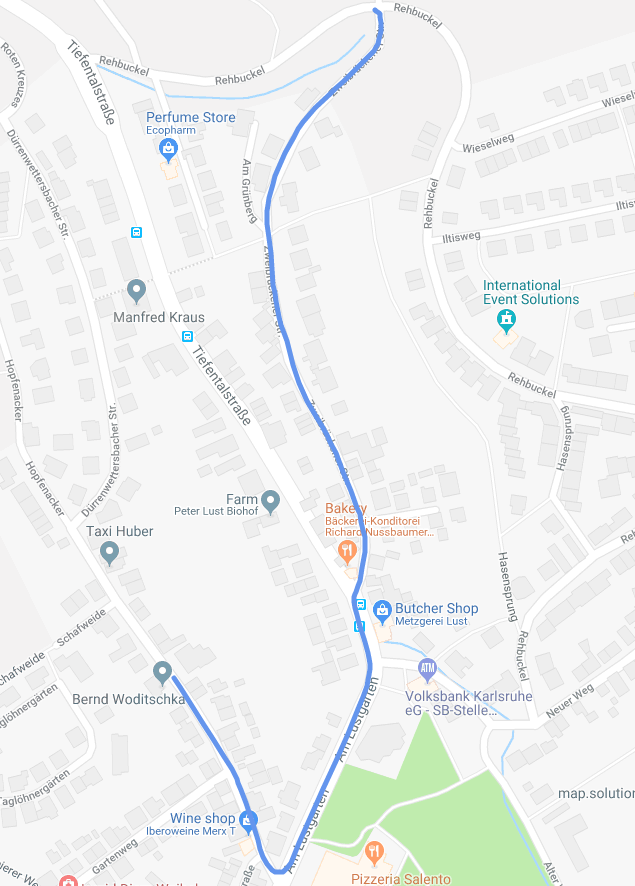
\includegraphics[scale=0.40,angle=90]{kitti_gps}
    \caption{The bird view of the KITTI test area. GPS trace was indicated blue line}
    \label{fig:kitti_gps}
\end{figure}
\noindent \textbf{Assessment of the Idea:} Since our aim is making an objective comparison, we benefit KITTI data and like in previous examples, we carried out same experiments and presented in figures \ref{fig:kitti_ndt}-\ref{fig:kitti_overall} and table \ref{tab:kitti_ndt}-\ref{tab:kitti}.
\par We, first, tested NDT algorithm with KITTI and observed that the behavior of obtained result almost the same as the previous example but with a slight difference. We assumed that the reason would be is the travelling velocity during the test drive, since our average speed was 10 km/h whereas their average speed was 20km/h. As a conclusion, we realized that after exceeding a certain limit of speed, it would cause discontinuity on localization. We also tested the other two methods ICP and combination of EKF with NDT and observed same behaviors once again. However, testing the EKF method was difficult than the previous example due to absence of wheel odometry so we could not thoroughly test EKF. Nevertheless, we presented its results even though its result was not satisfying.  
\par As a conclusion, we showed that NDT algorithm was the most successful methods among the other according to run different tests.
\begin{figure}[t]
    \centering
    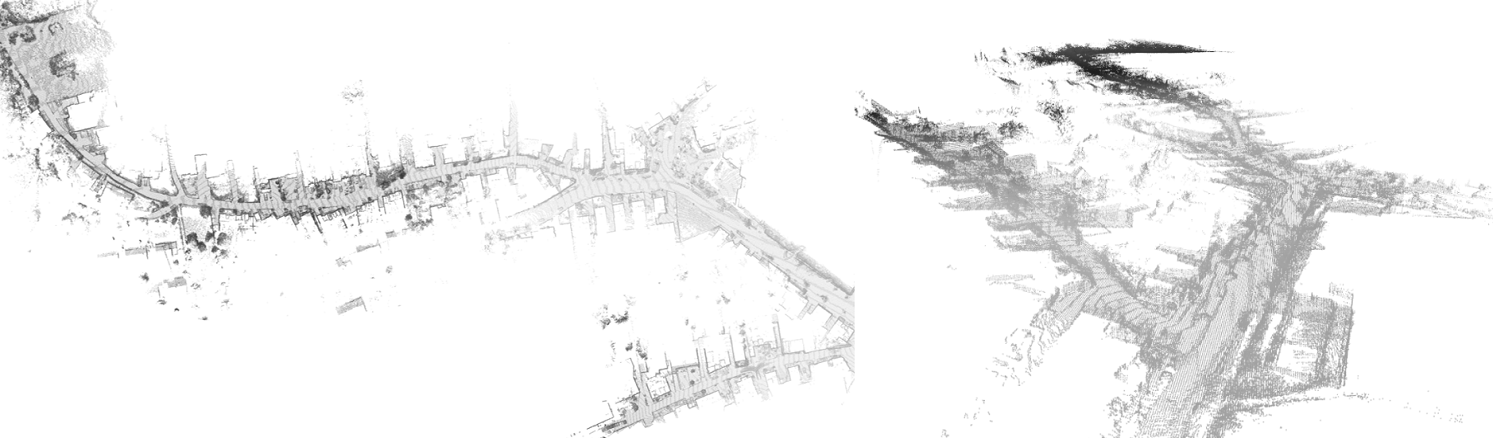
\includegraphics[height=7cm,width=\textwidth]{gray_kitti.png}
    \caption{3D map of KITTI sequence 10th test area which was constructed by NDT-algorithm}
    \label{fig:3D_kitti}
\end{figure}
\begin{figure}[H]
    \centering
    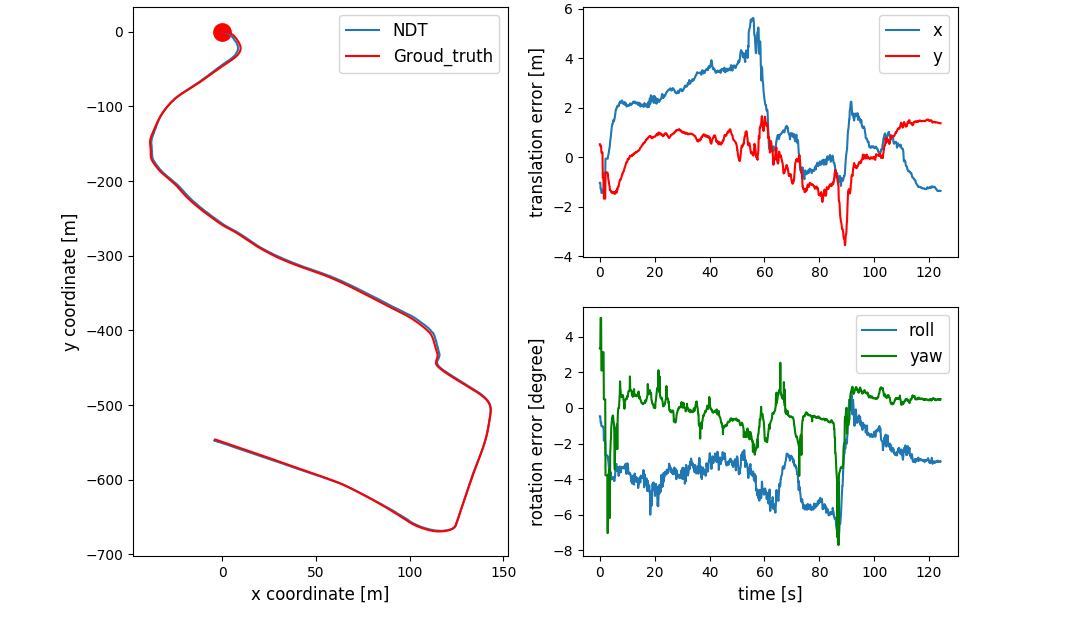
\includegraphics[height=7cm,width=\textwidth]{kitti_ndt_overall}
    \caption{Comparison between NDT and KITTI ground truth}
    \label{fig:kitti_ndt}
\end{figure}
\vspace{-0.5cm}
\begin{table}[H]
    \centering
    \small
    \begin{tabular}{|c|c|c|c|c|c|}
        \hline
         translation &max e.[m]&RMSE[m]&rotation&max e. [deg]&RMSE[deg]\\ 
         \hline
         x &5.63079  &2.24201   & roll   &-& -\\
         \hline
         y & 3.54759    &1.02374& pitch  & -& -\\
         \hline
         z &-          &-       &yaw& 7.71277 & 1.19939\\
         \hline
    \end{tabular}
    \caption{Error calculation data which was subtracted from figure \ref{fig:kitti_ndt}}
    \label{tab:kitti_ndt}
\end{table}

\begin{figure}[H]
    \centering
    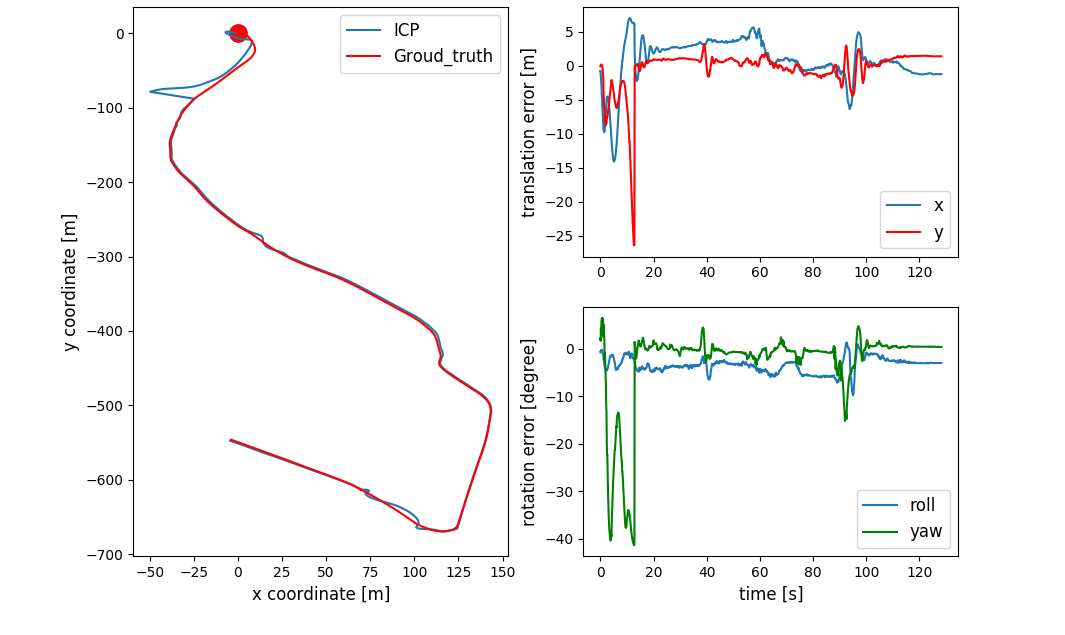
\includegraphics[height=7cm,width=\textwidth]{kitti_icp_overall}
    \caption{Comparison between ICP and KITTI ground truth}
    \label{fig:kitti_icp}
\end{figure}
\vspace{-0.5cm}
\begin{table}[H]
    \centering
    \small
    \begin{tabular}{|c|c|c|c|c|c|}
        \hline
         translation &max e.[m]&RMSE[m]&rotation&max e. [deg]&RMSE[deg]\\ 
         \hline
         x &14.0997  &3.36805   & roll   &-& -\\
         \hline
         y &26.42694    &3.14686 & pitch  & -& -\\
         \hline
         z &-          &- &yaw& 41.34196 &9.19015\\
         \hline
    \end{tabular}
    \caption{Error calculation data which was subtracted from figure \ref{fig:kitti_icp}}
    \label{tab:kitti_icp}
\end{table}

\begin{figure}[H]
    \centering
    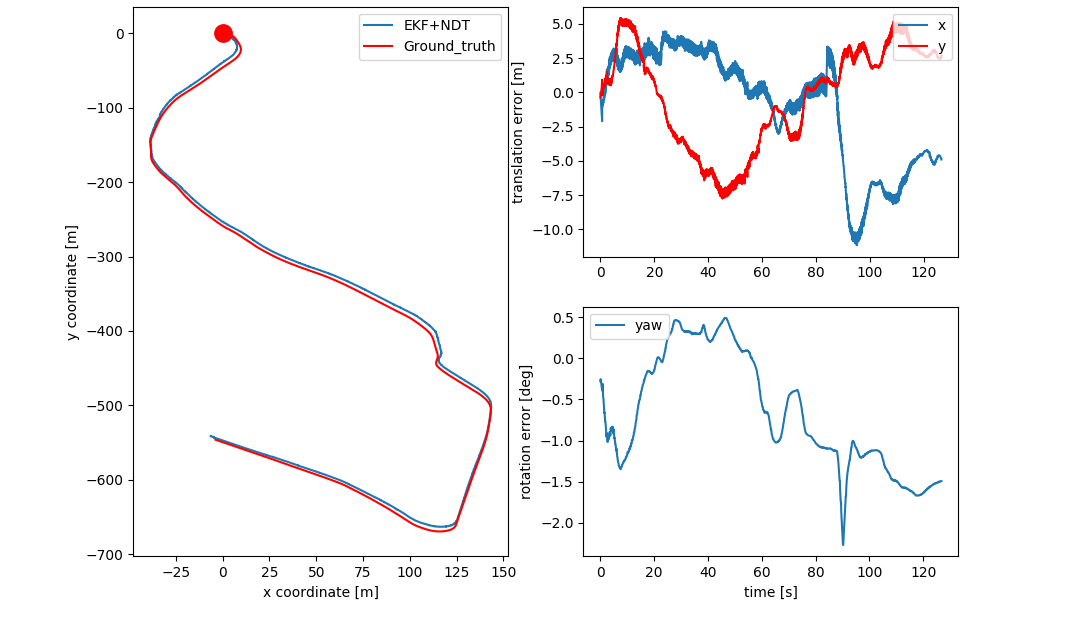
\includegraphics[height=6cm,width=\textwidth]{kitti_ekf_overall}
    \caption{Comparison between the combination of EKF with NDT and KITTI ground truth}
    \label{fig:kitti_overall}
\end{figure}
\vspace{-0.5cm}
\begin{table}[H]
    \centering
    \small
    \begin{tabular}{|c|c|c|c|c|c|}
        \hline
         translation &max e.[m]&mean e.[m]&rotation&max e. [deg]&mean e.[deg]\\ 
         \hline
         x &11.54453   &-0.88060  & roll   &-& -\\
         \hline
         y &6.82168    &-0.60853 & pitch  & -& -\\
         \hline
         z &-          &-       &yaw& 2.27149 & -0.67337\\
         \hline
    \end{tabular}
    \caption{Error calculation data which was subtracted from figure \ref{fig:kitti_overall}}
    \label{tab:kitti}
\end{table}

\section{Discussion}
Within the context of this thesis, several tests were performed and their results were presented in this chapter. However, there are some points need to be justified and discussed. We, here, would like to drag the attention of readers to these points. We expect that the combination of the EKF with NDT algorithm return more precise and smooth result. However, as shown in example \ref{sub:Bassum}, its result was somehow shifted to the right side of the ground truth. We believe that there are some reasons which cause this problem.  
\par The first reason would be a 3D map creation. Due to the inherent noise from LIDAR sensor, the accuracy of the map was not as perfect as ground truth. Therefore, it might cause a slight difference between the derived pose of the vehicle from scan matching methods and ground truth.
\par The second reason would be the absence of wheel odometry especially in case of KITTI data. Since there is no connection between the map and odometry which is explain in more detail in  REP-105\footnote{\url{http://www.ros.org/reps/rep-0105.html}}(conventions and semantic meaning for coordinate frames of mobile platforms used with ROS), it causes discontinuity, thus, EKF output had a discrete jump in order to converge true estimation.
\par Apart from these, in order to get a smoother result from these two scan matching algorithm, we would reduce the size of the voxel filter, by doing so, we would increase the overlap area and therefore, the estimated pose error decreases correspondingly the voxel size.

